\documentclass[letterpaper]{article}
\usepackage[pass]{geometry}

\usepackage{hyperref}
\hypersetup{colorlinks,urlcolor=blue}

\usepackage{tabularx}
\usepackage{array}
\usepackage{siunitx}
\usepackage{listings}
\usepackage{pdfpages}
\usepackage{color}

\definecolor{mygreen}{rgb}{0,0.6,0}
\definecolor{mygray}{rgb}{0.5,0.5,0.5}
\definecolor{mymauve}{rgb}{0.58,0,0.82}

\lstset{ 
  backgroundcolor=\color{white},   % choose the background color; you must add \usepackage{color} or \usepackage{xcolor}; should come as last argument
  basicstyle=\footnotesize,        % the size of the fonts that are used for the code
  breakatwhitespace=false,         % sets if automatic breaks should only happen at whitespace
  breaklines=true,                 % sets automatic line breaking
  captionpos=b,                    % sets the caption-position to bottom
  commentstyle=\color{mygreen},    % comment style
  deletekeywords={...},            % if you want to delete keywords from the given language
  escapeinside={\%*}{*)},          % if you want to add LaTeX within your code
  extendedchars=true,              % lets you use non-ASCII characters; for 8-bits encodings only, does not work with UTF-8
  frame=single,	                   % adds a frame around the code
  keepspaces=true,                 % keeps spaces in text, useful for keeping indentation of code (possibly needs columns=flexible)
  keywordstyle=\color{blue},       % keyword style
  language=C++,                 % the language of the code
  morekeywords={*,...},            % if you want to add more keywords to the set
  numbers=left,                    % where to put the line-numbers; possible values are (none, left, right)
  numbersep=5pt,                   % how far the line-numbers are from the code
  numberstyle=\tiny\color{mygray}, % the style that is used for the line-numbers
  rulecolor=\color{black},         % if not set, the frame-color may be changed on line-breaks within not-black text (e.g. comments (green here))
  showspaces=false,                % show spaces everywhere adding particular underscores; it overrides 'showstringspaces'
  showstringspaces=false,          % underline spaces within strings only
  showtabs=false,                  % show tabs within strings adding particular underscores
  stepnumber=1,                    % the step between two line-numbers. If it's 1, each line will be numbered
  stringstyle=\color{mymauve},     % string literal style
  tabsize=2,	                   % sets default tabsize to 2 spaces
  title=CAN Testbench                   % show the filename of files included with \lstinputlisting; also try caption instead of title
}

\lstset{basicstyle=\tiny}

\usepackage{graphicx}
\graphicspath{ {./images/} }

\title{Controller Area Network (CAN) and QFSAE}
\author{Ethan Peterson}
\date{\today}

\begin{document}

\maketitle

\section{CAN Bus Protocol}

\subsection{Background}
Controller Area Network (CAN) is a communications protocol that is standard for
electronics in the automotive industry. The protocol was introduced by the
Society of Automotive engineers (SAE) in 1986. CAN is primarily used for
communication between different electronics systems in different locations on
the car. For instance, sensor systems on the back of vehicle would be able to
read data from the Engine Control Unit (ECU). In the case of the team's car, the
ECU is the primary CAN device that other systems communicate with. The ECU
provides a variety of metrics about the engine such as RPM, throttle position,
ignition angle and many more. These metrics are read from the ECU over CAN by
using their CAN ID. Each message must have a unique ID from the IDs in use by
other devices on the car. It is also important to note that only one message can
be on a CAN bus at a time. Messages with more ``dominant" IDs will take
precedence on the bus. As a result, there must be careful consideration when
selecting an ID for a certain message depending on its priority overall.

\subsection{Data Transmission and Addressing}
CAN is two wire half-duplex serial based communication protocol. Half duplex
means that the CAN bus can only be used to send or receive messages in an
alternating fashion and not at the same time as with full-duplex protocols. CAN
messages consist of an identifier (CAN ID) and a data frame. There are several
standards for the size of the message frames. The ECU on the QFSAE car
implements the Society of Automotive Engineers (SAE) J1939 standard. This
standard uses 29 bit message identifiers and 64 bit data frames. Since CAN is
half-duplex, only one message can be on the bus at a time. However, CAN can
still be used to create large networks of CAN devices despite this through
its implementation of a priority bus. CAN defines ``dominant" and ``recessive"
bits where logical 0 is dominant. This allows to CAN to resolve conflicts on the
bus. The table below summarizes this process.

\begin{center}
  \begin{table}
  \begin{tabular}{c|c|c|c|c|c|}
    \cline{2-6}
      & \multicolumn{4}{c}{CAN ID Bits} & \\
    \cline{2-6}
      & Start Bit & 3 & 2 & 1 & 0\\
    \cline{1-6}
      \multicolumn{1}{|c|}{Node 3} & 0 & 0 & 0 & 0 & 1 \\
    \cline{1-6}
      \multicolumn{1}{|c|}{Node 4} & 0 & 0 & 1 & Stopped Transmitting & N/A \\
    \cline{1-6}
      \multicolumn{1}{|c|}{CAN Bus Data} & 0 & 0 & 0 & 0 & 1 \\
    \hline
  \end{tabular}
  \caption{
  \label{tab:Address Conflict Resolution}
    Demonstrating how CAN chooses the most ``dominant" ID on the bus in the
    case of a conflict between messages.
  }
  \end{table}
\end{center}

As a result of 0 being the dominant bit on the bus it is the smallest
CAN IDs that have the highest priority on the bus. This property of the bus must
be considered when selecting CAN IDs for custom messages outside of those
broadcast by the ECU. For example, a message indicating to the dash that a gear
shift happened is likely of a higher priority than updating the RPM.

\subsection{Wiring}
CAN consists of a two wire interface where the first two nodes connected to one
another should have two 120\si{\ohm} terminating resistors connected on either
end of the bus. Nodes are defined as devices connected to the bus which can send
or receive CAN messages. The diagram below is an example CAN network with three nodes.

\begin{center}
  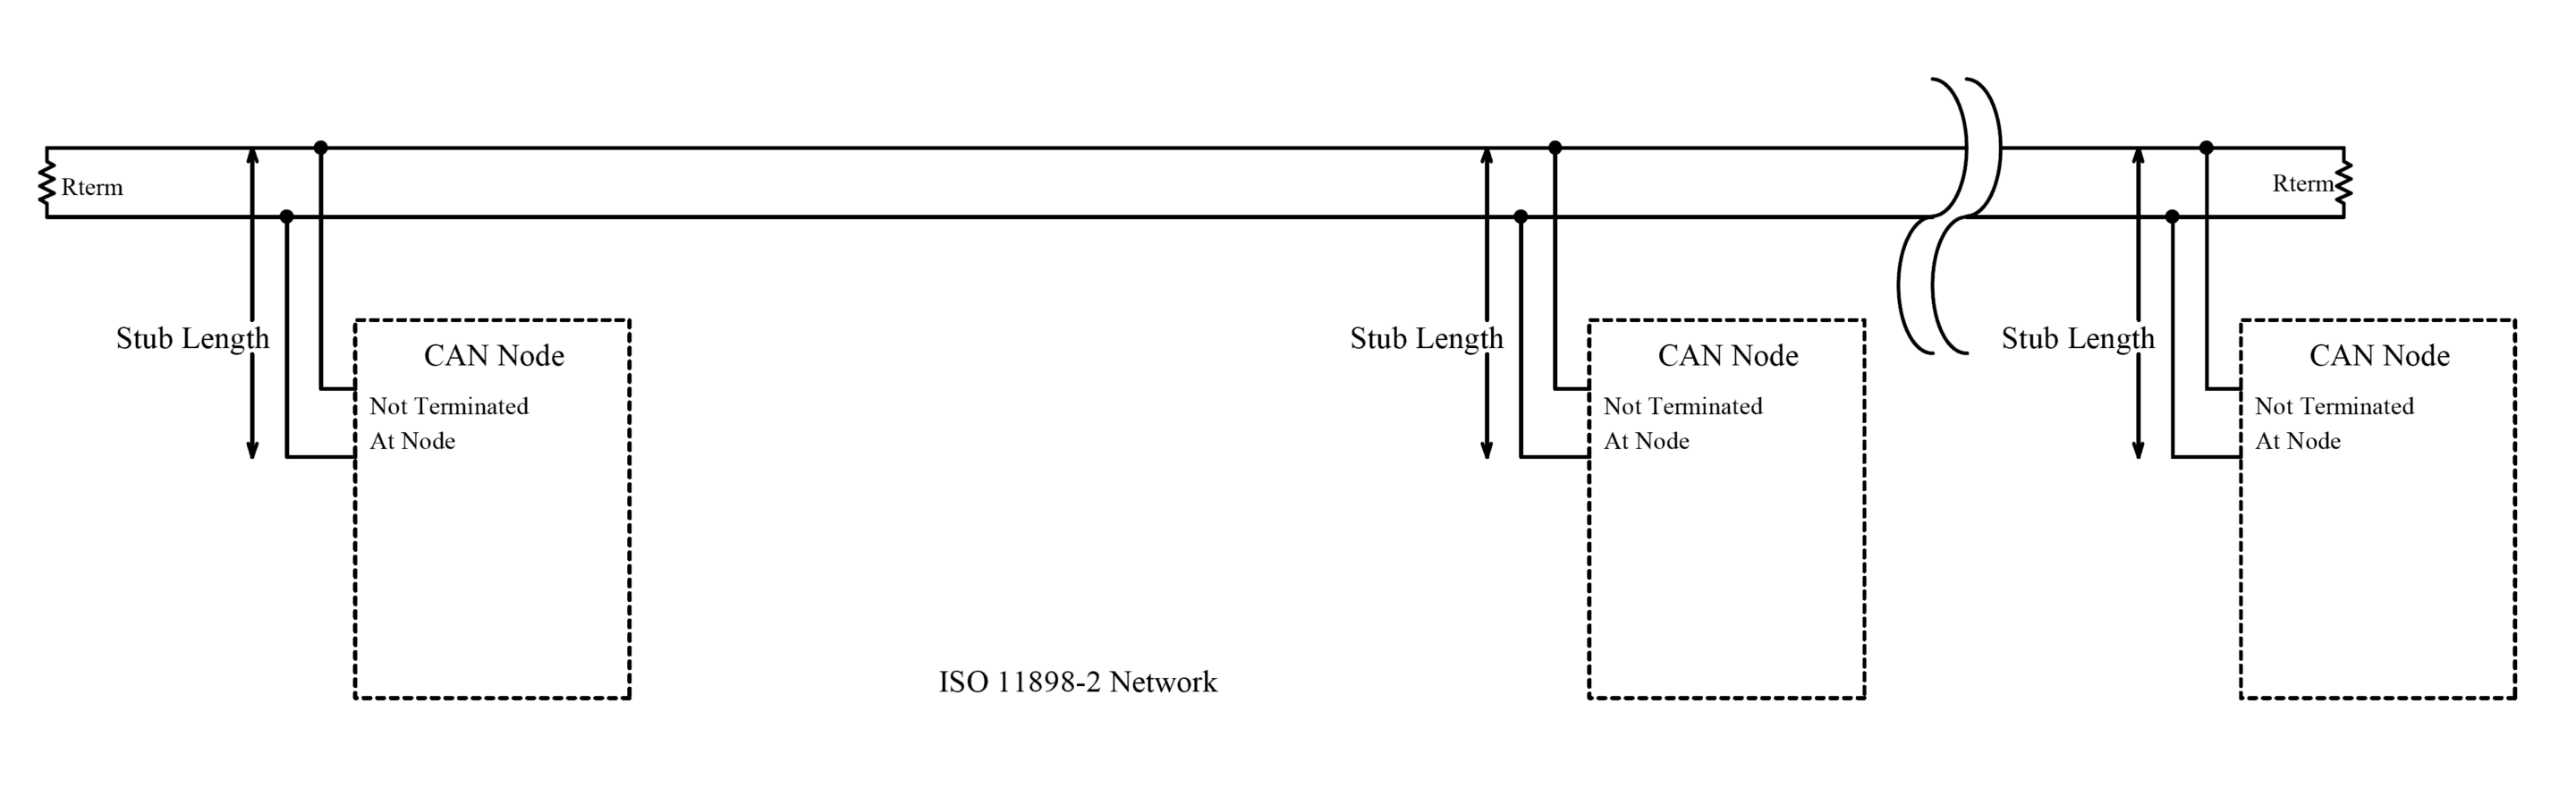
\includegraphics[width=\textwidth]{CAN-network-diagram}
\end{center}

\section{CAN on the Q19 Car}
In the case of the Formula car, The ECU has a terminating resistor and so does
the end of the car's CAN line where the CAN to USB dongle is found. Thus,
additional CAN peripheral should omit the terminating resistor to keep the bus
functioning properly.

\subsection{Testbench Code}
Given below is Arduino code for a CAN test bench. The Arduino INO file can be
found
\href{https://github.com/bchampp/Q20/blob/master/CAN/testbench/testbench.ino}{here}.

\lstinputlisting[language=C++]{../testbench/testbench.ino}

\lstset{basicstyle=\ttfamily}

The testbench code utilizes two Arduino Unos with CAN Bus shields to form a
two node network. \lstinline{SENDING} is a boolean value which determines whether the
Arduino will read or write data to the bus.

\subsection{Testbench Setup}
To get the CAN testbench up and running, the following items are required:


\begin{enumerate}
\item Two Arduino Uno Boards
\item Two Seeed Studio CAN Bus shields.
  \begin{itemize}
    \item Both CAN shield version 1.2 and version 2.0 implement the SAE J1939
      CAN standard used on the car.
    \item The code assumes a version 2.0 CAN shield is in use, if the CAN shield
      v1.2 is used then \lstinline{SPI_CS_PIN} definition should be set to 10.
    \item The shield versions can be told apart by the SD card slot that is
      present on v2.0 and absent on v1.2.
  \end{itemize}
\item USB Type B cable for programming.
  \begin{itemize}
    \item It is recommended that two cables are used such that the serial output
      from both Arduinos can be viewed concurrently for easier debugging.
  \end{itemize}
\item The Seeed Studio CAN Bus library, which can be installed
  \href{https://github.com/Seeed-Studio/CAN_BUS_Shield}{here}.
\item Two jumper wires for the CAN lines connecting the two shields.
  \begin{itemize}
    \item The instructions to connect the shields are on the
      \href{http://wiki.seeedstudio.com/CAN-BUS_Shield_V2.0/}{Seeed Studio Wiki}.
  \end{itemize}
\item Start the test bench by uploading the sender code to one Arduino and the
  receiver code to the other. The output can then be read from the Serial
  monitor.
\end{enumerate}

The configured testbench serves as a ``jumping off point" for other CAN related
and testing in a broader network. An important note about building CAN networks
using the test bench is to keep track of which nodes have a terminating
resistor. By default, both versions of the CAN Bus shield have terminating
resistors. Thus, nodes added to the same CAN bus should not have a terminating
resistor. In the case that a node with a terminating resistor is being added
(Ex. the ECU) then simply remove the terminating resistor from the CAN shield.
On shield versions 1.2 and 2.0 R3 is the terminating resistor. The figure below
shows the location of this resistor on both versions of the CAN shield. The
resistor is marked by a white rectangle.

\begin{center}
  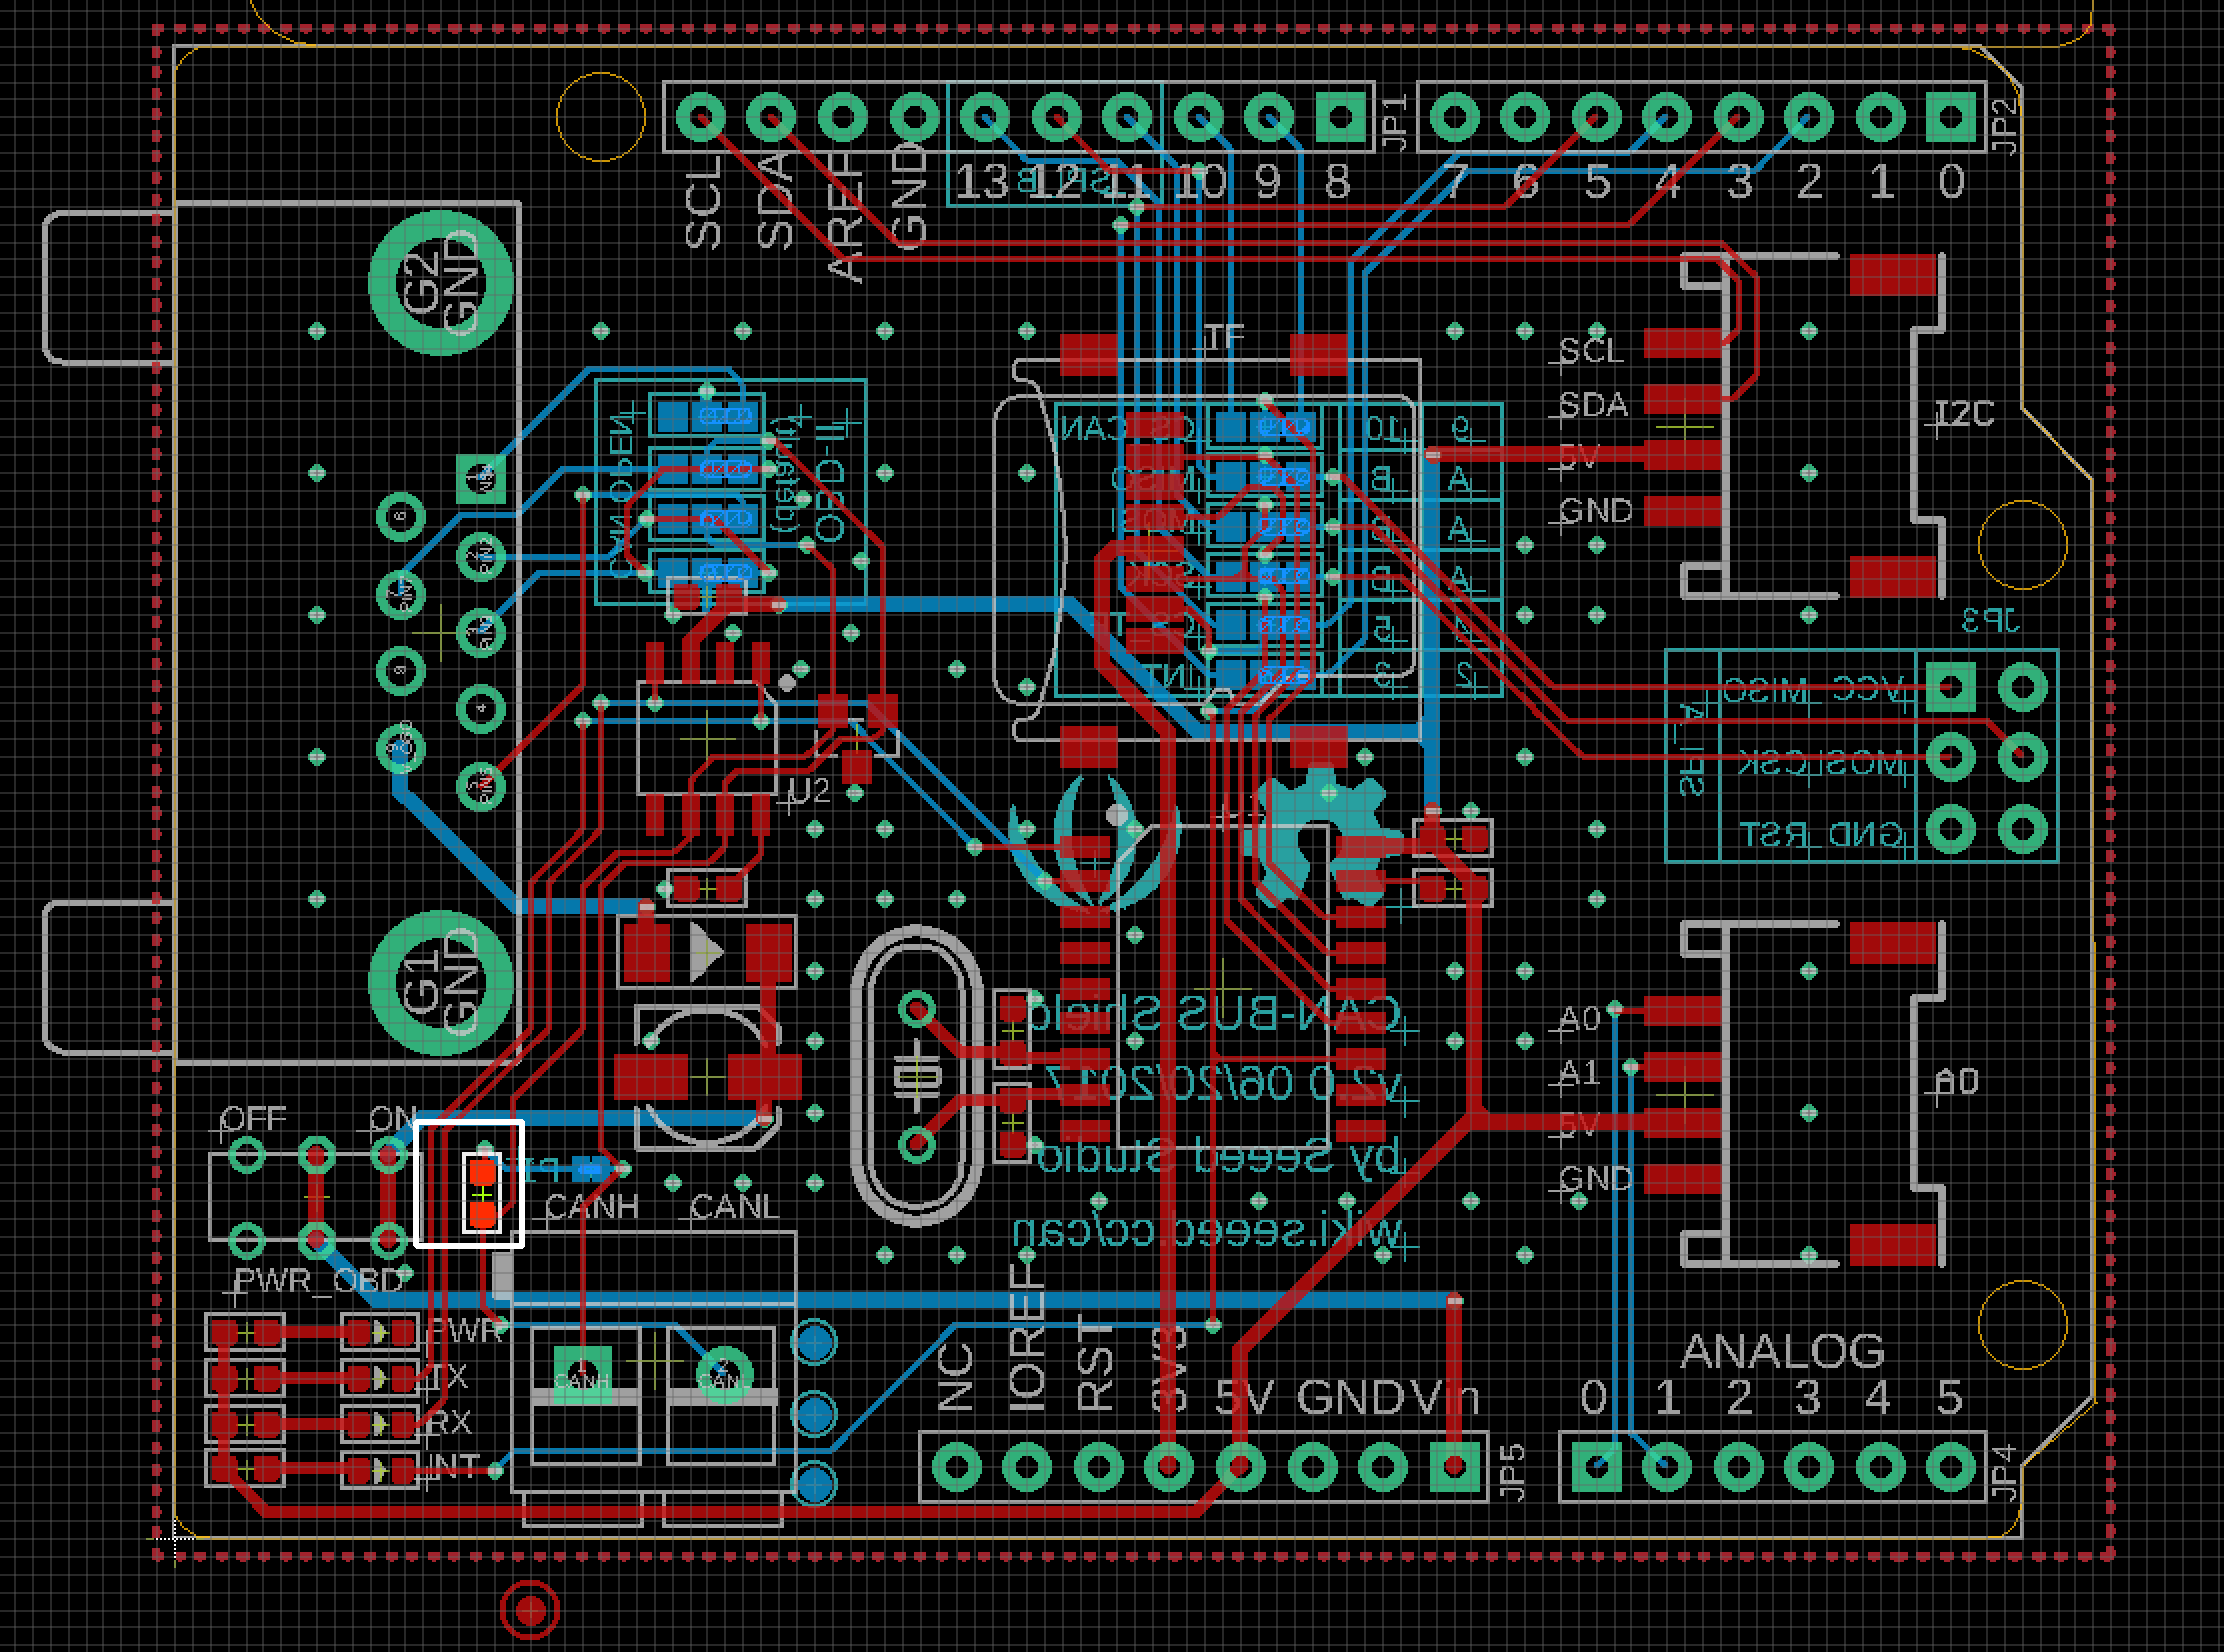
\includegraphics[width=\textwidth]{terminating-resistor}
\end{center}

\section{ECU Documentation}
Attached to the end of this document is an excerpt from the ECU datasheet which
gives a list of the CAN IDs and the contents of the data section of those
messages. This document should always be used as a reference when determining
priority of existing messages being sent over the bus and when selecting CAN IDs
for new messages.\\

TODO:
\begin{itemize}
  \item Document CAN library and retrieving ECU messages using the testbench.
\end{itemize}

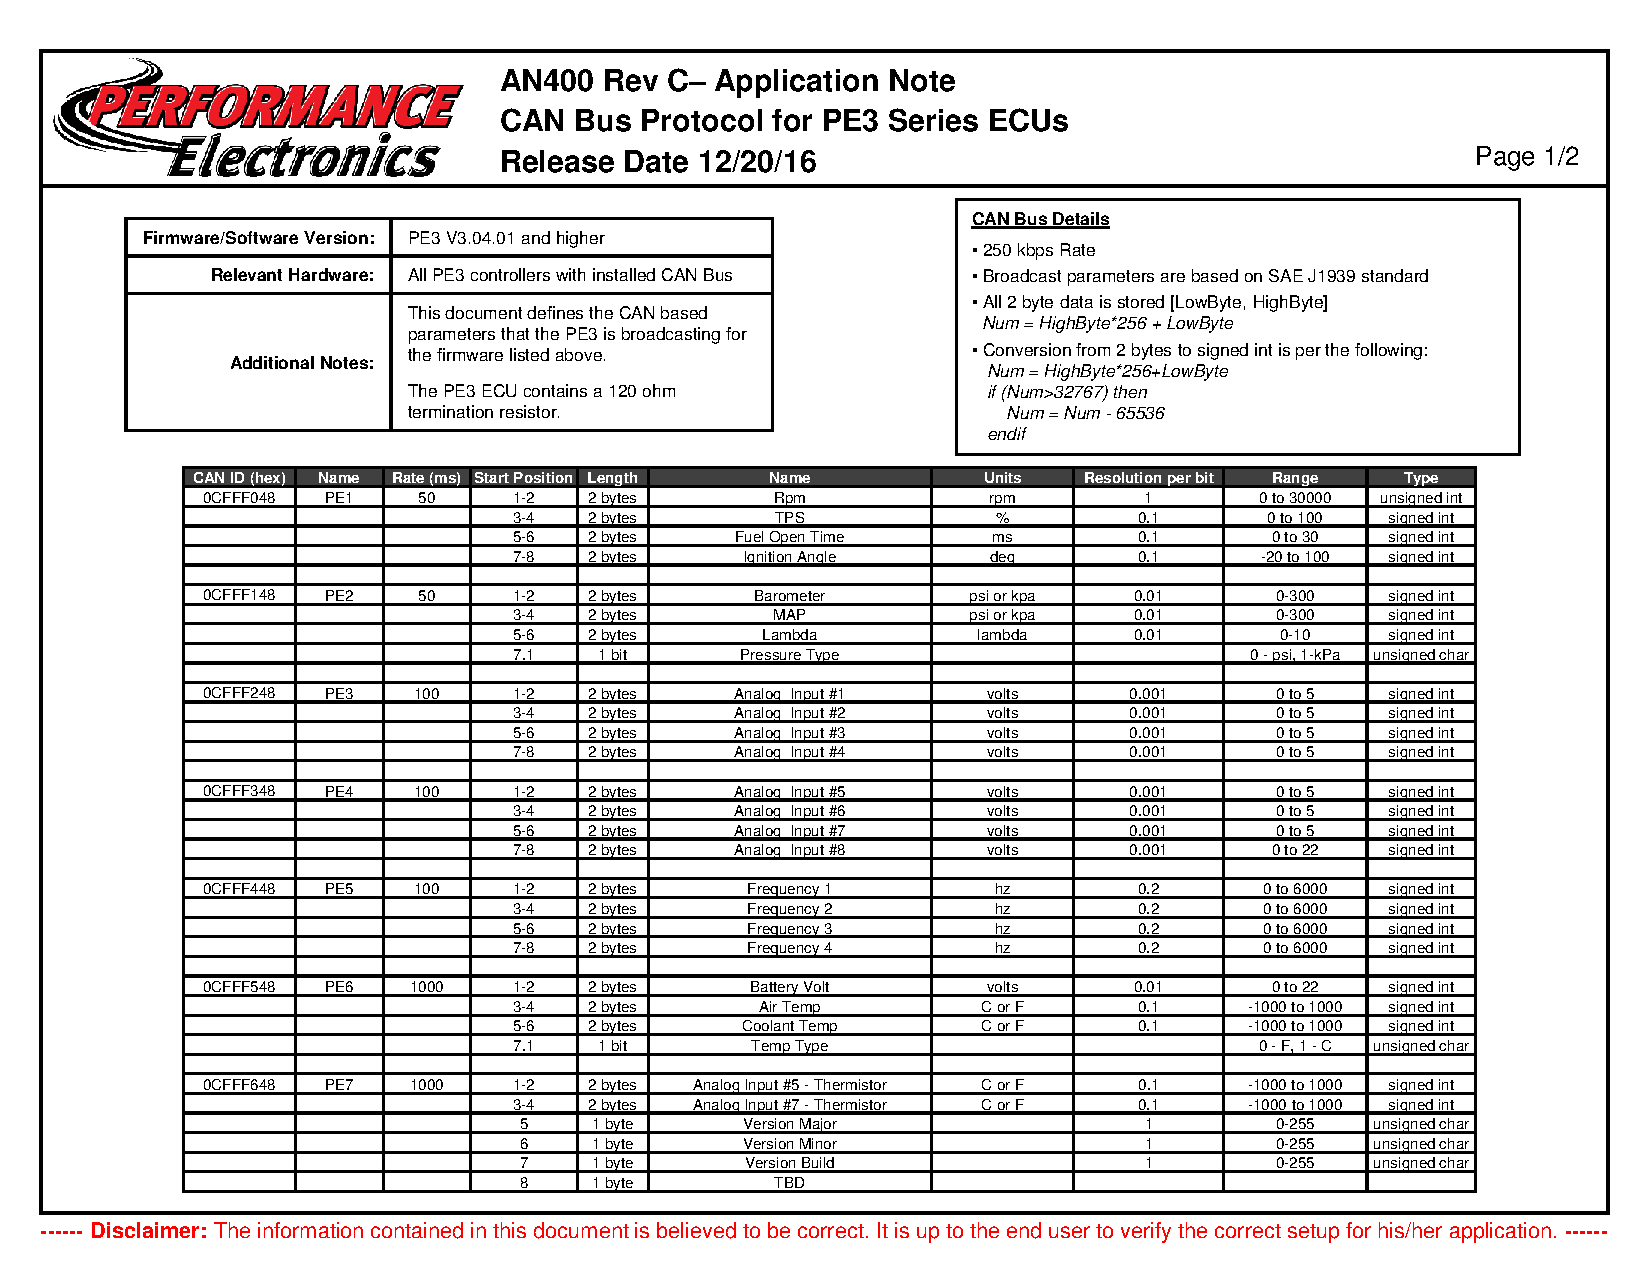
\includepdf[page = {1,2}]{PE3-ECU-CAN-Protocols}

\subsection{ECU Arduino Library}
QFSAE is developing a library to read these ECU message built atop the
CAN shield library.

\end{document}
